\section{Teorie barev}
Teorie barev by se dala popsat jako soubor postupů a pravidel zahrnující 
používání primárních pigmentových barev, vytváření barevné harmonie, míchání barev
a jejich aplikaci.

Abychom se však mohli věnovat samotným teoriím a určit postupy, se kterými budeme k této práci
přistupovat, je třeba začít s úplnmými základy a definovat si, co vlastně je barva a jak je vnímána
lidským okem.


\subsection{Barva}
Vnímání barev je velmi subjektivní a již od dob Aristotela nám jejich zkoumání nepřineslo
jednotný názor, který by přesně definoval barvu.
Ten založil své poznatky na pozorování slunečního světla, které při odrazu či průchodu objektem
snižuje svou intenzitu nebo je ztmaveno. Vnímal tak barvu jako mísení, míchání, superpozici či juxtapozici
černé a bílé~\cite{goethe1840}.

Tento názor se však později setkal s kritikou a byl nahrazen novými poznatky od dalších teoretiků. Dodnes je však
velmi dobrým základem pro další zkoumání vlastností barev.

\subsubsection{Isaac Newton}
S významným názorem přišel v 18. století významný fyzik, matematik, astronom a alchymista, Isaac Newton, ve své knize \emph{Optika}. Kniha dokumentuje Newtonovy pokusy s lomem světla
skrze hranol. Během svého pozorování objevil, že se jediný paprsek světla rozkládá do více barev v podlouhlém tvaru. V té době se jednalo o překvapující
objev. Dle přijatých zákonů lomu by mělo totiž rozptýlené světlo nabírat kruhovitých obrazců~\cite{adams2013newton}. Po dalších pozorováních vznesl Newton názor, že barva je 
viditelná část elektromagnetického spektra. Díky tomu můžeme rozeznávat různé barvy, ve svém spektru
identifikoval také konkrétní odstíny. Nejprve červenou, žlutou, zelenou, modrou a fialovou, později také oranžovou a indigo~\cite{science-color}.
Počet barev, tedy číslo 7, v tomto případě hraje významnou roli. Prvočíslo s mystickými významy udává také počet tónů na stupnici. A dle Newtona
právě tóny a sluch souvisel s barevným viděním. 

I přesto se ve své době nesetkal vždy s pozitivním ohlasem. Mnozí umělci stále věřili, 
že barva je něco mnohem komplexnějšího. Barvá má průhlednost, může být leská i matná, disponuje texturou i odstínem. Všechny tyto složky jsou důležitými aspekty, 
které nám dohromady vytváří svět tak, jak jej vidíme~\cite{gage2023colour}.

\begin{figure}[!htbp]
    \centering
    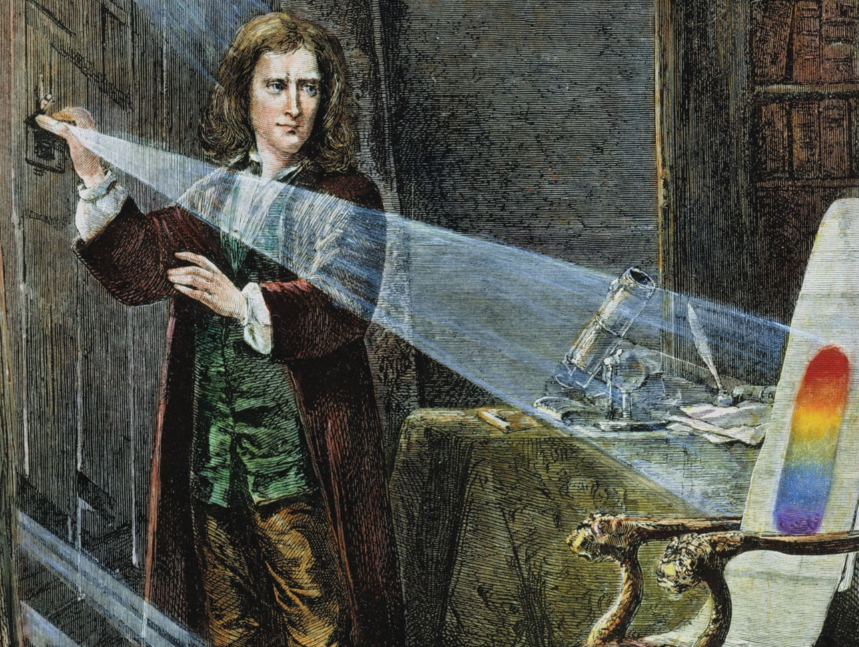
\includegraphics[width=0.7\linewidth]{images/sir_newton.png}
    \caption{Sir Isaac Newton experimentující s hranolem. Rytina dle obrázku od J.A. Houston, ca. 1870. Se svolením The Granger Collection, New York~\cite{sirIsaacNewton}}
    \label{fig:Sir Isaac Newton}
\end{figure}

\subsubsection{Johann Wolfgang von Goethe}
Jedním z těch, kteří barvu chápali jako mnohem abstraktnější pojem, byl německý spisovatel Johann Wolfgang von Goethe. Důležitým dílem se stala kniha \emph{Teorie barev}, kde Goethe zpochybňuje
Newtonovy názory. V jeho spisu popisuje barvu ne jako vědecký údaj, ale jako subjektivní zážitek, přírodní vjem projevující se kontrastem, mísením, zvětšením či dělením.
Součástí díla je taktéž první systematická studie o fyziologických účincích barev. 

Goethe rozdělil barvu do tří tříd podle toho, jak
se projevují. První jsou psychologické barvy, které závisí na oku a reakci orgánů. Dalšími jsou fyzické barvy, ty jsou produkovány materiálními médii, avšak sami o sobě barvu mít nemusí. Jejich vnímání je určené okem, a to 
prostřednictvím vnějších vjemů či odrazů. Tyto barvy jsou pomíjivé a nelze je zadržet na dlouhou dobu. Třetí třídou jsou chemické barvy, které patří daným látkám a jsou trvalé po libovolně dlouhou dobu~\cite{goethe1840}.


Goetheovo definování barev je založeno spíše na jeho zkušenosti a ve své knize se zaměřuje na vnímání psychologické a emocionální.
Ačkoliv z lidského pohledu jeho tvrzení nejsou nekorektní, postrádají fyzikální základ a nesoustředí se na vědecké vlastnosti. 

\subsubsection{Young-Helmholtzova teorie}
Jen o pár desítek let později vznikla nová, dodnes v praxi využívaná teorie. Základ ji dodal anglický vědec Thomas Young v roce 1802, který
příšel s \emph{trichromatickou teorií barevného vidění}. Nespokojil se totiž s Newtnovým názorem o velkém množství částic v oku a vytvořil
předpoklad, že existují tři fotosenzitivní receptory reagující na základní barvy, tedy červenou, modrou a zelenou. Drážděním receptorů pak 
vznikají další barevné kombinace a spojením všech tří vznikne dojem bílé barvy. Jejich absence pak vytváří dojem černé.

Myšlenku následně rozvedl německý fyziolog Hermann Ludwig Ferdinand von Helmholtz. Dle jeho poznatků nejsou receptory drážděny pouze jednou barvou,
ale všemi třemi s různou intenzitou. Tak mohou vznikat všechny možné barevné odstíny a drážděním všech tří barev ve stejném poměru vytváří vjem bílé.
Té lze ale dosáhnout také smícháním dvou komplementárních barev (např. modré s oranžovou).

Tuto teorii podpořili i další osobnosti, jedním z nich je Ragnar Granit. V roce 1964 Paul K. Brown a George Wald prokázali existenci tří fotopigmentů sítnice citlivé
na různé vlnové délky, později Ragnar Granit, Haldan Keffer Hartline a George Wald dokázali existenci těchto fotoreceptorů spektrofotometrickým vyšetřením
absorpce světla. Za tento objev získali v roce 1967 Nobelovu cenu~\cite{vackova2013teorie}.

Tato teorie je využívána dodnes, dle některých zdrojů známá pod názvem \emph{Young-Helmholtz-Maxwellova teorie}. Skotský fyzik, James Maxwell, se totiž v době Helmholtzova zkoumání věnoval stejnému
tématu a rozšiřoval tuto teorii o další pozorování. Potvrdil existenci tří typů receptorů a popsal barvoslepost jako poruchu těchto receptorů. Zároveň definoval světlo jako
elektromagnetické vlnění a popsal souvislosti vlnových délek s barvou světla~\cite{958782}.


\begin{figure}[!htbp]
    \centering
    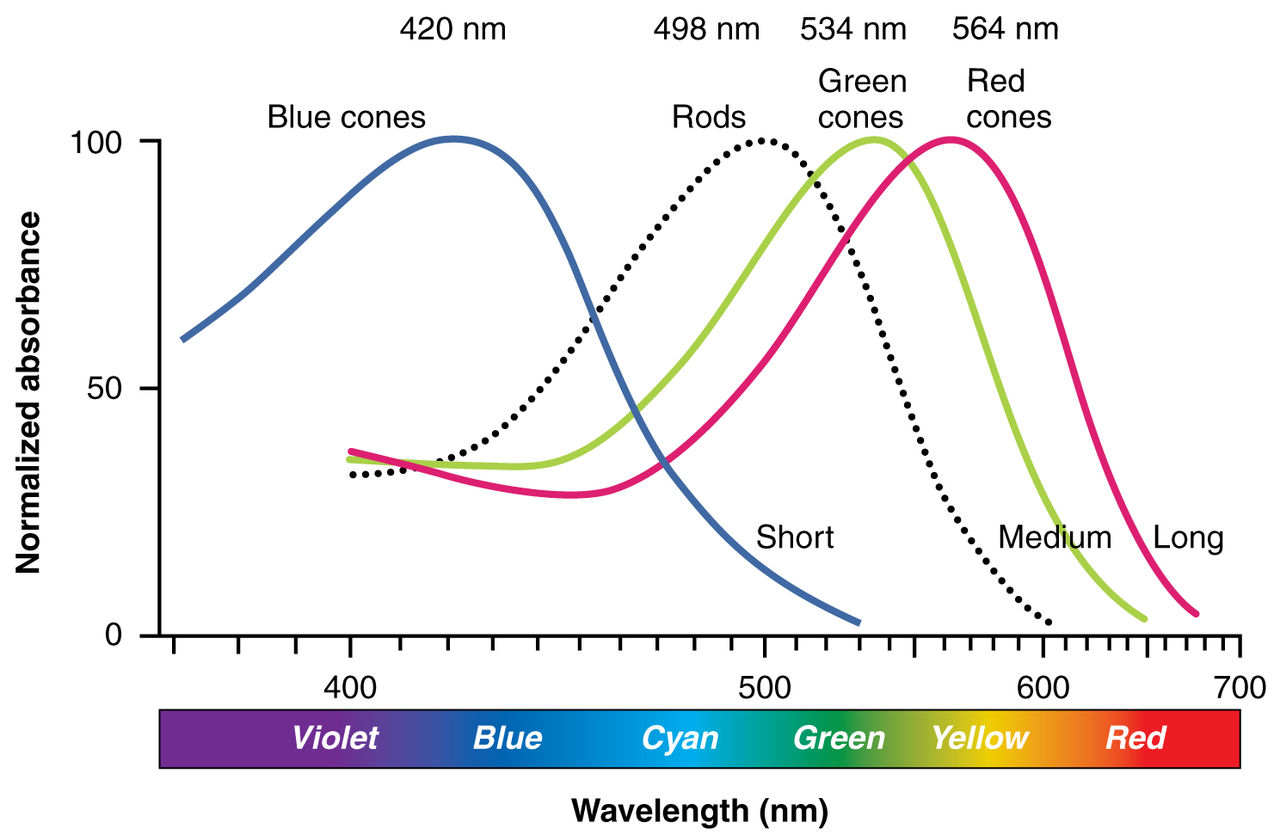
\includegraphics[width=0.7\linewidth]{images/Color_Sensitivity.jpg}
    \caption{Spektrální absorpční křivky pigmentů krátkých (S), středních (M) a dlouhých (L) vlnových délek v lidských čípkových a tyčinkových (R) buňkách.~\cite{cone-response}}
    \label{fig:Spektrální křivky}
\end{figure}

% Newton, Maxwell, Young, Goethe - zkoumání barev (goethe1840)
% https://library.si.edu/exhibition/color-in-a-new-light/science
% https://books.google.cz/books?hl=en&lr=&id=mujNEAAAQBAJ&oi=fnd&pg=PP13&dq=colour+definition&ots=ECMtqQBf1F&sig=-kCLAYmN6owutngTKMQAJ4Fu2fc&redir_esc=y#v=onepage&q&f=false
% https://d1wqtxts1xzle7.cloudfront.net/112207887/jaic_v32_01-libre.pdf?1709866938=&response-content-disposition=inline%3B+filename%3DColour_theory_Definition_fields_and_inte.pdf&Expires=1752252945&Signature=ZfOn9uc-IsbJP3TrC5MvZV4lSsAOte25rIBlngEMk7LidfCjxXVDtY9tmgN8RPonzWEm4AD0TRa-vkG0SGxMuVksHhNWawTge-7yJNuDxPnS5vOLtoCdWxS3Qpb1Uj1qdG~UnhJq8XXZFIubw9iDNmgUWR0fhSkD~ejasDRYdj-~ZjkHxcYEVLaazY~OFY3QhmTVcZ25B1bzPfnxpwZjDOMPBVPJX397~6qY~0ZsyctLy0jzs8ehTZahxoXmJz8vCDESfASXwe~4IDfXkmWs-2u1JjHVFVDsWb-HVVp~witzDU-VBO0odEnlIta0~WRoEeWiA6oyjz893LdCmRO8iw__&Key-Pair-Id=APKAJLOHF5GGSLRBV4ZA
% další research pro historii a vývoj názorů, odkud a co je barva 
% https://www.pantone.com/articles/color-fundamentals/what-is-color#:~:text=Color%20is%20defined%20as%20the,others%20are%20absorbed%20by%20it.
% pantone stránka - moderní definice barvy, dnešní chápání 

\subsubsection{Vlastnosti barev}
% odstín, sytost a jas - https://dspace.cuni.cz/bitstream/handle/20.500.11956/188964/130380558.pdf?sequence=1
% odstín - název barvy
% sytost - množství šířeného světla, jak moc obsahuje barva bílou
% jas - intenzita barvy, kolik světla vychází z barvy
Pro pochopení, co je barva, je třeba znát i vlastnosti barev, které popisují jejich vzhled a charakterizují je. Definují se nejčastěji numericky vzhledem k faktu,
že lidské oko jej objektivně vyhodnotit nedokáže. Základními atributy barev jsou odstín, sytost a jas~\cite{jelen2023vliv_barev}.

\paragraph{Odstín}
Odstín je vyznačován názvem konkrétní barvy. Liší se v závislosti na vlnové délce a je rozhodující pro výslednou podobu barvy. Další atributy vzhledem k jejich
podstatě totiž fungují pro diskriminaci barev spíše jako doplňkové.

\paragraph{Sytost}
Sytost určuje množství bílé v konkrétní barvě. Čím větší množství bílé barvy obsahuje, tím menší je sytost. Udávána je nejčastěji v procentech, kde 0 \% značí černobílou a 100 \% 
plnou sytost bez černého či bílého pigmentu.

\paragraph{Jas}
Jas určuje světelnou intenzitu barvy, tedy množství světla vycházející z dané barvy. Více světelných paprsků vytváří světlejší vjem barvy. Stupnice pro měření jasu je od 0 do 100, kde 0
značí absolutní černou. Lidské oko je údajně schopno rozlišit až 300 stupňů jasu barev v různých odstínech.


\subsubsection{Moderní definice}
Jak tedy definovat barvu na základě veškerých zmíněných poznatků? Obecně lze říci, že barva je aspekt způsobený kvalitou světla odrážejícího se či pohlceného daným objektem.
Abychom viděli barvu, je třeba mít světlo. Lidské oko zvládne vidět pouze barvy, které se odráží nebo reflektují. Samotné vnímání však zůstává stále velmi subjektivní~\cite{pantone}.

\subsection{Oko a barevné vidění}
Oko je smyslový orgán reagující na světlo, který nám zajišťuje zrak. Díky očím můžeme vnímat naše okolí, vidět a rozeznávat barvy
v závislosti na jejich vlnové délce. Oko je složené z rohovky, duhovky, čočky, sklivce, zrakového nervu a stínice.
Právě sítnice je zodpovědná za barevný vjem. Jedná se o průhlednou blanku, jenž je rozdělená linií ora serrata. Přední část
neobsahuje žádné smyslové či nervové elementy, v zadní části se nachází světločivé buňky - tyčinky a čípky. Těch je v sítnici
přibližně 130 milionů~\cite{hanulikova2013}.

\paragraph{Tyčinky}
Tyčinky jsou mnohem početnějším typem fotoreceptoru než čípky. Jsou taktéž mnohem citlivější, při optimálních podmínkách je dráždí i jednotlivé
fotony. Tyčinky zajišťují černobílé vidění a umožňují nám adaptovat se na tmu. Převládají v periferním vidění, které je díky tomu citlivější na světlo.
Jsou složeny ze zevního a vnitřního segmentu, které spojuje zúžená část. Pod tímto zúžením se nachází bazální tělísko s nahromaděnými mitochondriemi
v jeho okolí, jejichž existence je důsledkem zvýšené produkce energie, jenž je důležitá pro proces vidění. 

\paragraph{Čípky}
Čípky jsou strukturované podobně jako tyčinky. Zevní segment je však kratší, silnější v kónickém tvaru.
Tvar se může lišit i dle jejich lokality na sítnici, v centrální jamce, místě nejsotřejšího vidění, mohou být i delší než tyčinky. Nejvíce jich pak lze nalézt v 
žluté skvrně. Čípky, stejně jako tyčinky, obsahují zrakový pigment. Narozdíl od tyčinek osabující pouze jeden typ pigmenut, přesněji purpur,
mají však rovnou tři typy tohoto pigmentu. Dělí se dle vlnových délek na krátké S (short), středně dlouhé M (medium) a dlouhé L (long). Jsou citlivé na modré, zelené a červené světlo. 
\\
\begin{figure}[!ht]
    \centering
    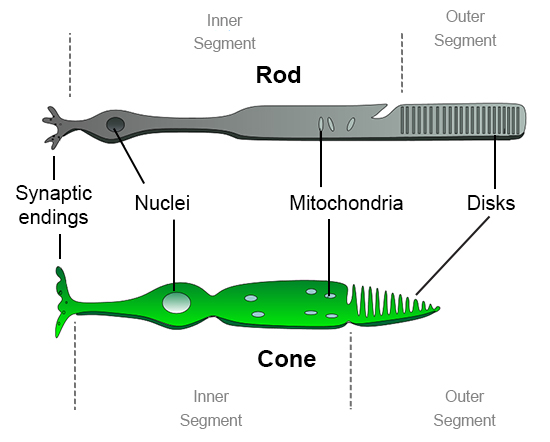
\includegraphics[width=0.6\linewidth]{images/rods-cones.jpg}
    \caption{Struktura tyčinek a čípků v oku.~\cite{RodsAndCones}}
    \label{fig:Tyčinky a čípky}
\end{figure}
\\
Při vstupu světla do oka prochází postupně nejprve rohovkou, přední oční komorou s tekutinou, následně prostorem se sklivcem až do sítnice. Fotoreceptory pohlcují světlo
spolu s velkým množstvím enzymů a molekul přeměňující světelnou energii na kinetickou energii. Tento chemický proces vytváří nervový vzruch a následně se šíří až do mozku.
Samotný mechanismus vnímání barev dodnes není úplně jasný, v dnešní době je však nejrozšířenější dříve zmíněná Young-Helmholtzova teorie. Spolu s Heringovou teorií, dle které
využíváme dva protikladné páry pro vnímání barev - červenou a zelenou s žlutou a modrou, tvoří
Dvoustupňovou teorii kombinující oba názory, která je dnes akceptována vědci~\cite{soukup2020}.

% https://is.muni.cz/th/gpxge/Diplomova_prace.pdf
% struktura oka, tyčinky - černobílé, čípky - barevné vidění, proces předávání informace do mozku
% https://www.mendeley.com/catalogue/a9dda4be-621f-3d6f-b83d-343556b66070/
% trichromatické vidění - long(reddish), medium (greenish), and short (bluish) vawelenghts
% https://dspace.cvut.cz/bitstream/handle/10467/91222/FBMI-BP-2020-Soukup-Jan-prace.pdf?sequence=-1&isAllowed=y
% teorie vnímání barev,  Young-Helmholtzova - tři typy čípků, Heringova teorie - proces
% spojení obou teorií - Dvoustupňová

\subsubsection{Vliv kontextu na vnímání barev}
Již víme, že oko obsahuje velké množství fotoreceptorů umožňující nám vidět v barvách. Ne vždy se na něj však lze spolehnout a v rámci vidění jsme limitování různými aspekty,
dle nichž se mohou některé věci jevit rozdílně. Kontext zde hraje důležitou roli.

Při segregaci objektů je důležité nejen to, co vidíme, ale také vyhledávání v paměti mezí tím, co již známe.
Barva slouží k identifikaci objektů a stavu objektu. Banán rozeznáme díky jeho žluté barvě, stejně tak zvládneme díky barvě
rozeznat citron od limetky. Barva, kterou si pamatujeme díky zkušenosti s konkrétním objektem, se nazývá \emph{paměťová barva}.
Barevně neutrální jsou pak objekty bez této paměťové barvy, příkladem mohou být například auta, u kterých si jedinou barvu nelze spojit.

Kromě rozpoznávání objektů ovlivňuje paměťová barva i naše vnímání. Tento vliv se nazývá \emph{Efekt paměťové barvy}. Dle tohoto efektu se nám
mohou objekty jevit zbarvené do určitého odstínu i přesto, že jsou vyobrazeny pomocí stupnice šedi. Černobílý banán se nám tak stále může jevit jemně
nažloutlý. Naopak pro dosažení černobílého vjemu je třeba úprava barvy směrem k opačnému odstínu. Například namodralý obrázek banánu se tak bude jevit
spíše černobílým.

\begin{figure}[!ht]
    \centering
    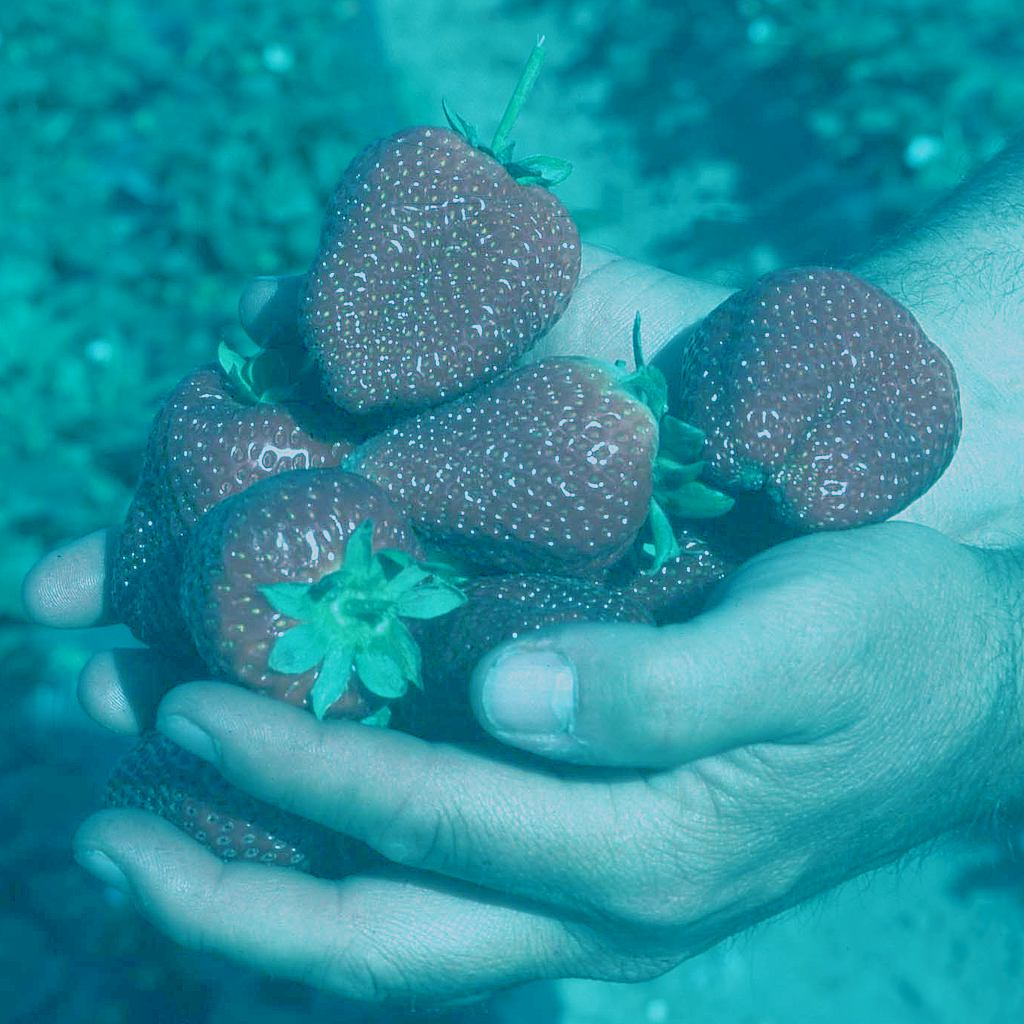
\includegraphics[width=0.35\linewidth]{images/Strawberries_memory_colour.jpg}
    \caption{Paměťová barva jahod rozpoznatelná i tehdy, když je jejich fotografie zmanipulována tak, že červená barva je šedá.~\cite{memory-colour-strawberries}}
    \label{fig: Paměťová barva}
\end{figure}

Vliv paměťové barvy se ukázal nejsilnějším u modrých a žlutých odstínů. Jedním z důvodů se jeví proměnlivost denního světla. Právě žlutá s modrou
odpovídají přirozenému dennímu světlu, což může způsobit nejistotu od pozorovatele~\cite{color-perception}.
\\
\\
Důležitým efektem kontextu na vnímání barev je také kontrast. Fenomém barevných stínů popisuje nasvícení
bílé obrazovky dvěma světly. První světlo dlouhé vlnové délky vypadá červeně, druhé světlo působí bíle. Dle
očekávání se obrazovka bude jevit červeně. Při posazení objektu do cesty pak vzniknou dva stíny. První stín se
zablokovaným zdrojem bílého světla se jeví sytě červeně, druhý stín se zablokovaným červeným světlem se však jeví nazelenale.

\begin{figure}[!ht]
    \centering
    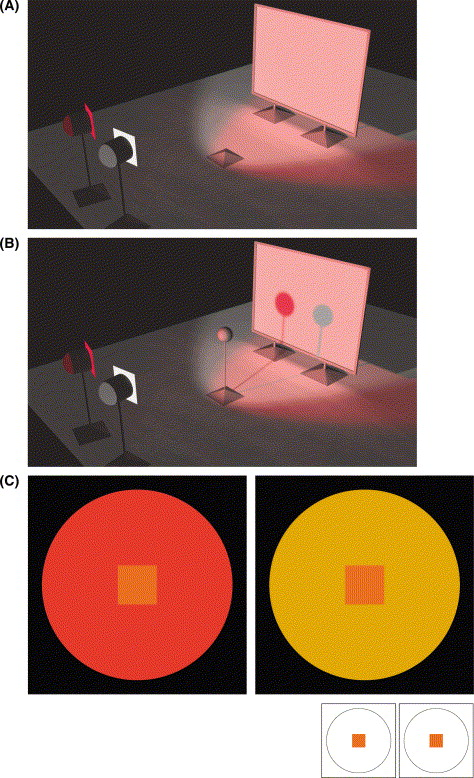
\includegraphics[width=0.65\linewidth]{images/contrast.jpg}
    \caption{Příklady barevných stínů a vlivu pozadí na vnímání barvy objektu.~\cite{BEAULOTTO2002609}}
    \label{fig:Kontrasty}
\end{figure}

O tento jev se zajímal francouzský chemik Chevreul, který následně vydal spis popisující pravidla kontextu na vnímání barvy.
Dle jeho poznatků je vnímaná barva objektu vychýlena směrem k opačné barvě pozadí na Newtonově barevném kruhu. Tento efekt byl hojně
využíván v umění i průmyslu~\cite{BEAULOTTO2002609}.
\\
\\
I věk hraje roli v kontextu vnímání barev. S vyšším věkem je člověk náchylnější k poruchám vidění a hůře rozeznává barvy. Nejen vyšší věk
je však důvodem zhoršeného barevného vidění. Studie ukazují, že u novorozenců dochází k postupnému vývinu čípkových kanálu, tedy zpočátku
rozeznávají pouze velmi syté a dostatečně velké objekty s určitým odstínem. I v pozdějším věku se však vnímání stále vyvíjí a saturačního prahu
na úrovni dospělého je dosaženo pravděpodobně až v pozdní adolescenci~\cite{infant-perception}.

% https://www.annualreviews.org/docserver/fulltext/vision/4/1/annurev-vision-091517-034231.pdf?expires=1752399604&id=id&accname=guest&checksum=25D512DF5FD9FEB5457EB71FA73304F5
% memory color effects - objekty spojené s určitou barvou (banán - žlutá) ovlivňují vnímání - objekt na šedém spektru vnímán jinak
% The empirical basis of color perception - https://www.sciencedirect.com/science/article/pii/S1053810002000144
% kontrast - pozadí barev, jiné vnímání
% věk - https://srcd.onlinelibrary.wiley.com/doi/full/10.1111/cdep.12447
% novorozeňata - horší barevné rozlišování, menší saturace
%maybe oslnění

\subsection{Vliv barev v běžném světě}
Vnímání barev není jen prostředkem pro rozeznávání objektů a vyhodnocování stavů daných objektů. Díky barevným vjemům můžeme
prožívat emoce, ovlivňovat naše nálady a aktuální stav či upevňovat sociální nastavení. Díky vhodné volbě barevných prvků lze
manipulovat člověkem ke koupi produktu, či například k volbě politické strany.
\paragraph{Test zelené barvy}\mbox{}\\
Existují například studie, které sledovaly účinek zelené barvy jako primitivní rys přírodních prostředí na výsledky cvičení a změnu
nálad. Z pozorování vyplynulo, že oproti například červenému či achromatickému filtru zeleň snižuje narušení nálady spolu s hodnocením
vnímání obtížnosti cvičení. Naopak pocit hněvu byl silnější u červeného filtru~\cite{Akers2012}.
% nálada, sociální postavení, aktuální stav: vzrušení, klid, stres, i chut
% https://pubs.acs.org/doi/abs/10.1021/es301685g - test zelené
\paragraph{Vliv barev na chování spotřebitele}\mbox{}\\
Další studií zkoumající vliv barev v běžném světě se věnuje ovlivňování barev na chování spotřebitele. Zde je kladen důraz na rozlišování
barev primárně dle zkušenosti. Tedy na rozdíly mezi teplými a studenými tóny, zářivými a tmavými odstíny a jejich asociaci s náladou. 
Studené tóny v lidech probouzí větší klid, tmavé odstíny jsou přirovnávány k negativnímu kontextu, smutku a nudě, naopak zářivé odstíny jsou vnímány jako hravé, 
radostné a plné naděje.

Zálěží však také na původu spotřebitele, věku i vzdělání. Američtí konzumenti jsou přitahování k modré a červené, naopak občané Íránu a Kuwaitu
preferují modrou se zelenou. Občané ve vyšším věku jsou méně otevřeni experimentování s barvami a u vzdělanějších osob probíhá výběr barev mnohem složitějším
způsobem. Zakomponování teorie barev v konzumní společnosti je tedy náročný úkol, kterým se zabívají mnozí experti. I přes komplikovanost úkolu
jsou totiž výsledky velmi efektivní. Design balení a výběr barev totiž mají nejen signifikantní vliv na samotnou koupi produktu, ale také vytvoření asociace
s produktem, díky které si lze zákazníka udržet~\cite{consumer-behavior}.
% https://link.springer.com/chapter/10.1007/978-3-319-91716-0_32 - ovlivnovani barev na chovani zakaznika

\subsection{Poruchy barevného vidění}
Ačkoliv je pro většinu z nás zcela přirozené vidět barvy, i přes jejich subjektivní vnímání, v plné kráse, barevné vidění není samozřejmostí pro každého.
Barvoslepost je porucha, při které dochází k omezení rozeznávání barevných tónů, a to buď částečně, či dokonce úplně. Následující kapitola je převzata a upravena na 
základě bakalářské práce Kláry Holišové (2007), která se komplexně věnuje problematice barevného vidění~\cite{Holisova2007thesis}.

\subsubsection{Vrozené poruchy barevného vidění}
Při úplné barvosleposti vnímá postižený svět jako černobílý film. V některých případech je schopnost rozeznávat barvy zcela omezena, v některých případech pouze oslabena.
Budeme se řídit příponami, kde \emph{-anomálie} značí oslabení a \emph{-anopie} úplnou barvoslepost. Předpona \emph{prot-} pak označuje vadu pro vnímání červené barvy, \emph{deuter-} pro vnímání zelené a \emph{trit- }
pro vnímání modré. Osoby se správným vnímáním všech tří barev jsou označování \emph{trichromati}, ti, kteří disponují poruchou barevného vnímání, se nazývají \emph{dichromati} a \emph{monochromati}.
%file:///C:/Users/sarka/Downloads/Barevne_videni_Archive.pdf
% dichromati, monochromati 
% prot-, deuter-, tri- (vady dle barvy - červená, zelená, modrá) - anopie vs anomálie
\paragraph{Anomálie}\mbox{}\\
Rozlišujeme tři typy anomálií. Protanomálii způsobuje nedostatečné množství červených čípků, postižený špatně rozlišuje mezi červenou a zelenou. Touto anomálií trpí
až 1 \% mužů. Nejrozšířenějším typem anomálie je deuteranomálie, která se týká také zhoršeného rozeznávání červené a zelené z důsledku oslabení zelených čípků. Postihuje
až 5 \% mužů. Tritanomálie je vzácnější porucha, při které dochází k zhoršenému rozeznávání žluté a modré barvy. Není vázána na pohlaví, tedy postihuje ve stejné míře muže
i ženy.

\paragraph{Dichromati}\mbox{}\\
Jak již bylo zmíněno, dichromati jsou osoby se schopností rozlišovat pouze odstíny vzniklé ze dvoz základních barev. Jeden z čípků chybí. Protanopie značí poruchu vidění
červené barvy, postižení zaměňují červenou za zelenou, špatně také rozeznávají rozdíly mezi modrou a zelenou. Deuteranopie je poruchou vidění zelené barvy. V tomto případě dochází k zaměňování
zelené až modré za fialovou. Tritanopie je, stejně jako tritanomálie, nejvzácnější z těchto tří poruch. Jedná se o poruchu vidění modré barvy.

\paragraph{Monochromati}\mbox{}\\
Monochromati disponují jediným typem čípků a nedokáží rozlišit barvy. Vidí v odstínech šedé, zvládnou rozlišit pouze intnezitu světla.

\begin{figure}[!ht]
    \centering
    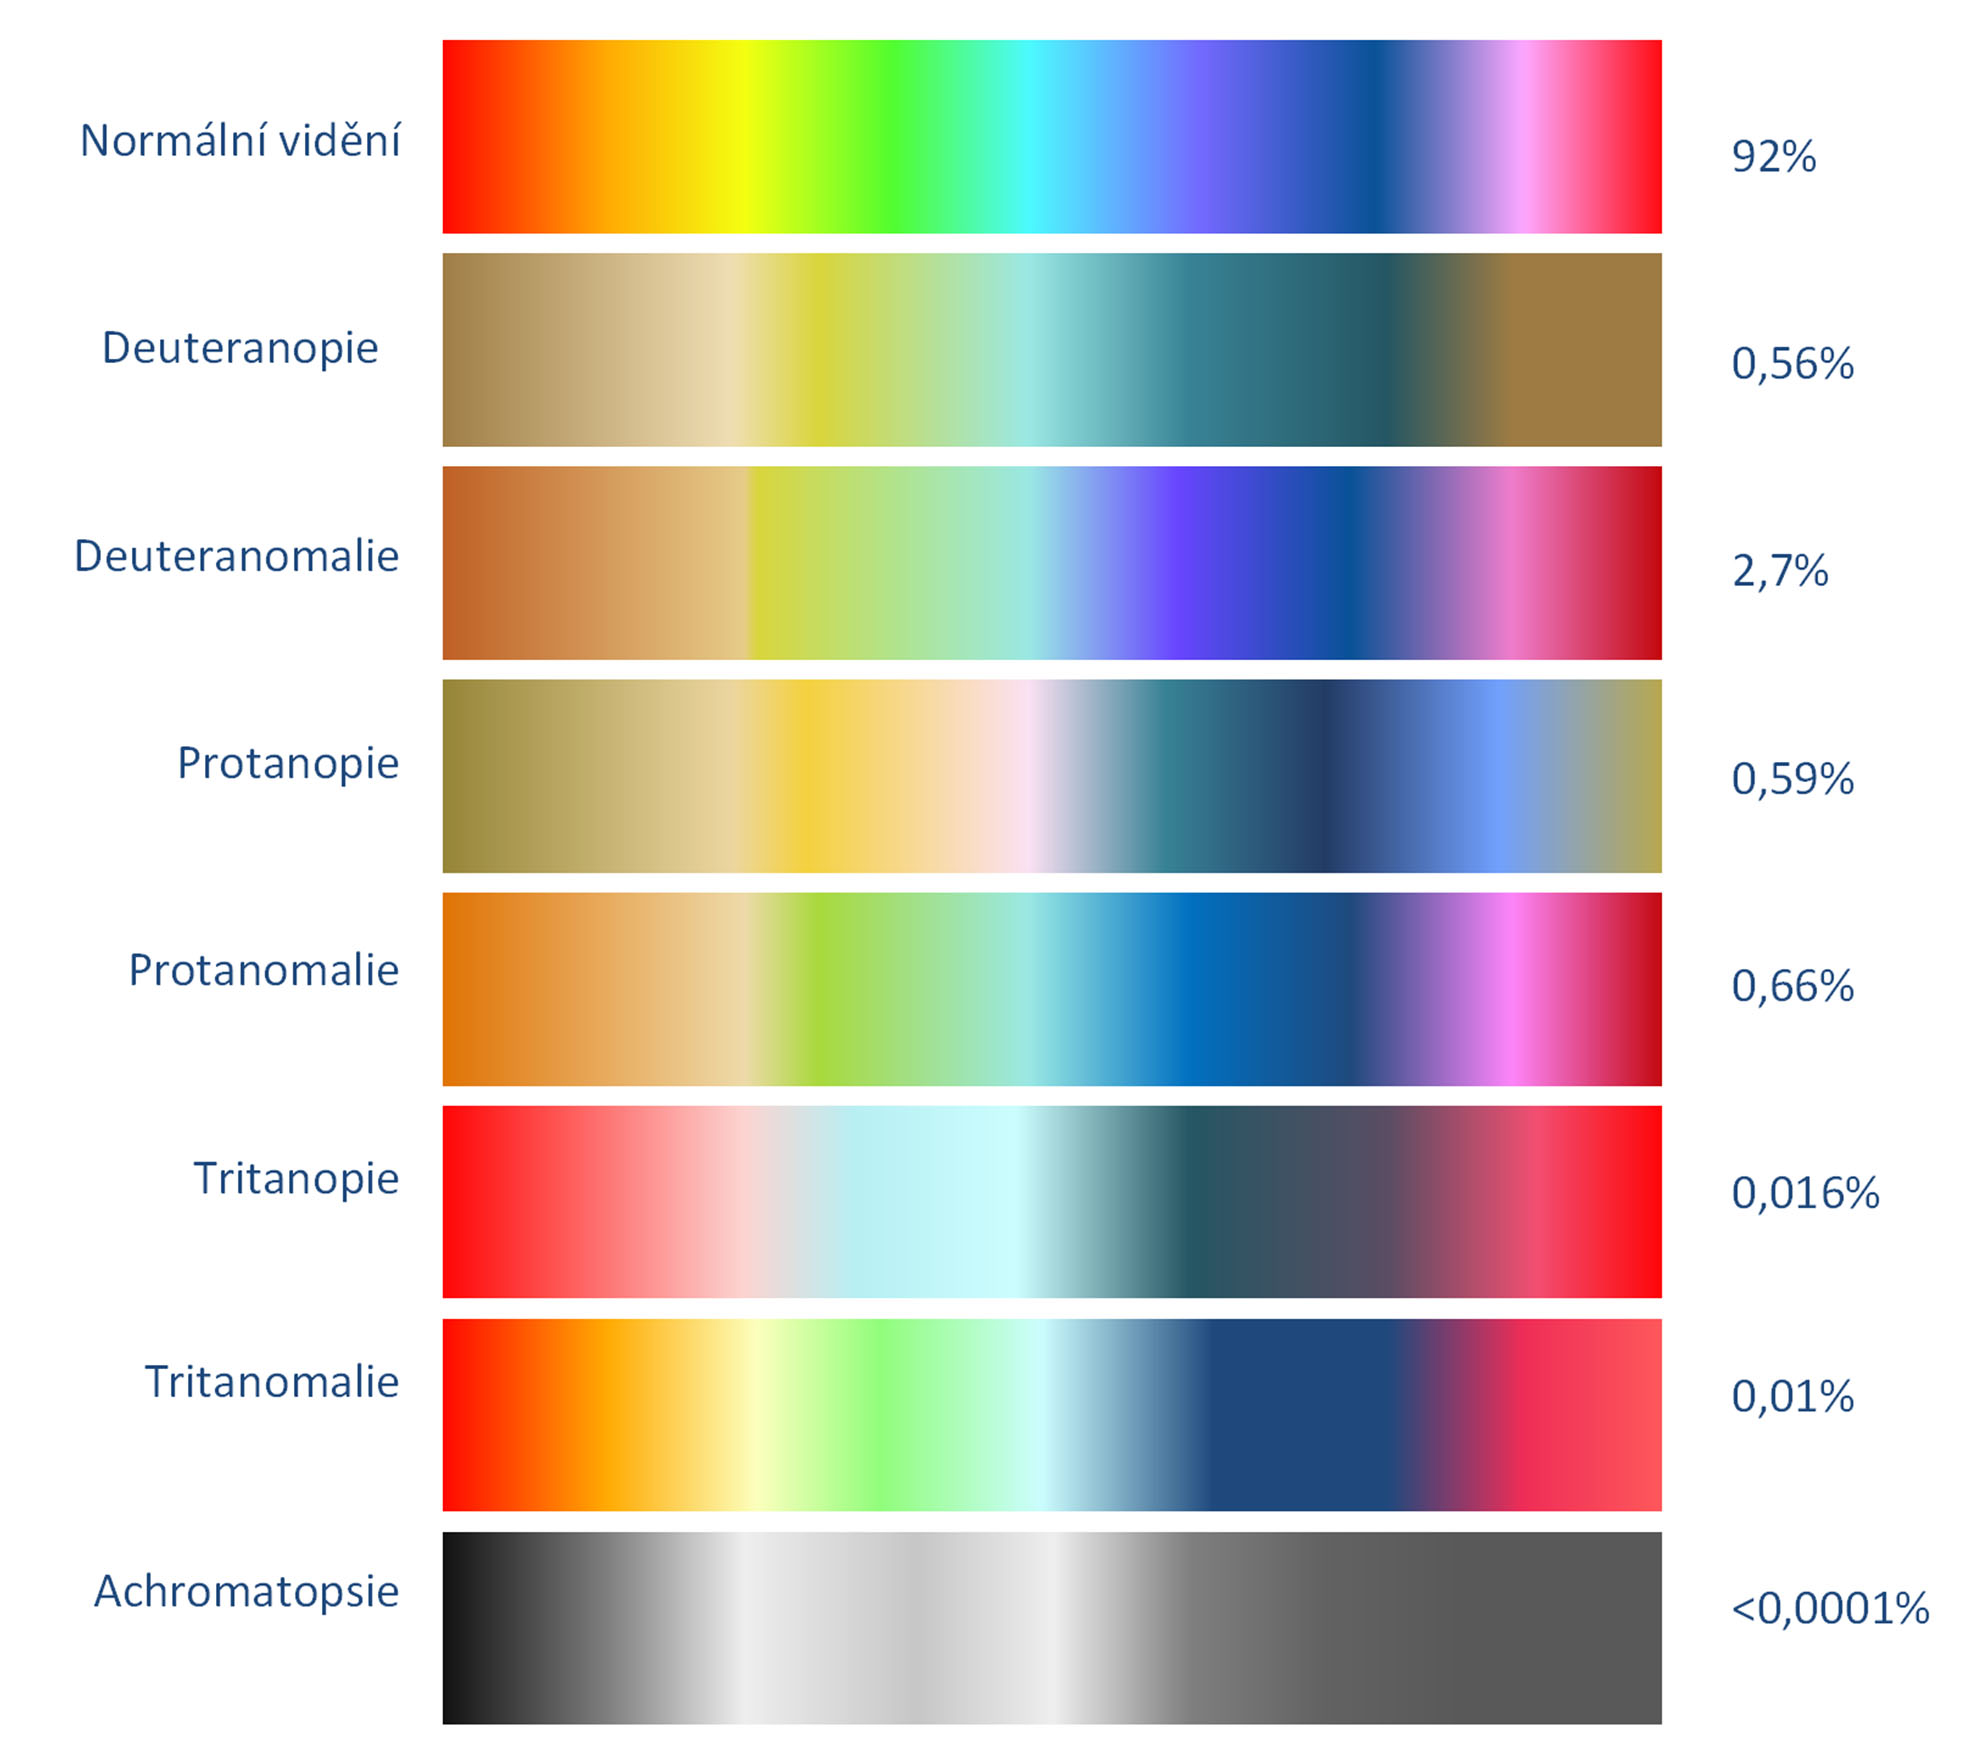
\includegraphics[width=\linewidth]{images/spektra-poruchy.jpg}
    \caption{Vnímání spektra viditelného světla u zdravých osob a osob s poruchami barvocitu, 
    včetně informace o procentuálním výskytu poruch barvocitu v populaci.~\cite{10.1145/2632048.2632091}}
    \label{fig:Vnímání}
\end{figure}

% katarakta (šedý zákal)
% Achromatopsie - poškození mozkových center
% chromatopsie - nepřirozeně barevné vidění, užíváním drog
\subsubsection{Získané poruchy barevného vidění}
Kromě vrozených poruch existují také poruchy získané. Ty jsou nezávislé na pohlaví, typicky bývají asymetrické mezi očima a méně stálé než choroby vrozené. 

Katarakta, neboli šedý zákal, je choroba, při které má oční čočka sklon ke žloutnutí. Následkem žloutnutí absorbuje krátkovlnné světlo a zhoršuje se rozeznávání
v modré oblasti spekra. Šedý zákal se rozvíjí v důsledku stárnutí, ale nejedná se o jediný faktor přispívající k jeho vzniku. Přispět může také například
vystavení oka nepřiměřenému infračervenému záření, rozvinout se může také důsledkem traumatu či systémového onemocnění, jako je diabetes mellitus či galaktosemie.

Achromatopsie je vzácná porucha způsobená poškozením mozkových center, které zodpovídají na zpracování barevného vjemu v čtvrté vizuální oblasti temporálního
laloku. Tato část je zodpovědná za zpracování barev a tvarů a je důležitá pro rozeznávání objektů. Vzniká důsledkem kyslíkových poruch, například při otravě oxidem uhelnatým
či při mrtvici.

Důsledkem Chromatopsie je nepřirozené vnímání barev. Rozlišují se dle viděných barev na cyanopsii pro modrou, chloropsii pro zelenou, erythropsii pro červenou a xantopsii
pro žlutou barvu. Vzniká při dlouhodobém užívání drog, kataraktou, nebo například při oslnění světlem. 

\subsection{Teorie barev}
% https://app.knovel.com/kn/resources/kpCDTAE004/toc - historie
% teorií existuje mnoho, zmínit nejznámější:
% Aristoteles
% Isaac Newton
% Goethe
% Tobias Mayer
% JOHANNES ITTEN
% JOSEF ALBERS
%https://library.si.edu/exhibition/color-in-a-new-light/science#:~:text=Aristotle%20developed%20the%20first%20known%20theory%20of,until%20being%20replaced%20by%20those%20of%20Newton.
%https://web.mit.edu/22.51/www/Extras/color_theory/color.html

